\documentclass[a4paper, twocolumn]{article}
\newcommand{\papertitle}{Whitepaper: Community Development of Next Generation Storage and Compute Interfaces}

\usepackage[a4paper, margin=2cm]{geometry}

\usepackage[utf8]{inputenc}
\usepackage[T1]{fontenc}
\usepackage{graphicx}
\usepackage[english]{babel}
\usepackage[colorlinks=true,urlcolor=red]{hyperref}
\usepackage{url}
\usepackage{cleveref}

\usepackage{multicol}
\setlength{\columnsep}{1cm}

\usepackage{fancyhdr}
\fancyhead{}
\fancyfoot{}
\fancyhead[l]{\papertitle}
\fancyhead[r]{
\includegraphics[height=1em]{ngi-logo}}
\fancyfoot[r]{\thepage}
\pagestyle{fancy}
\renewcommand{\headrulewidth}{1pt}
\renewcommand{\footrulewidth}{1pt}

\usepackage{titling}
\pretitle{\begin{center}\Large\bfseries}
\posttitle{\end{center}\vskip 0.5em}

\graphicspath{{./assets/}}

\title{\papertitle}

\author{Julian M. Kunkel \\
  \textit{University of Reading}
	\and
  A
  \and
  B
  \and
  C
}
\date{\today}


\begin{document}
\maketitle
\thispagestyle{fancy}

\section*{Abstract}

The efficient, convenient, and robust execution of data-driven workflows and enhanced data management are key for productivity in scientific computing and computer-aided RD\&E.
Big data tools integrate compute and storage capabilities into a holistic solution demonstrating the benefit of tight integrating while the HPC community still optimizes the compute and storage components independently from each other, and, moreover, independently from the needs of end-to-end workflows from users that lead to the final insight.
Utilizing a homogeneous storage and compute infrastructure efficiently is complex for experts even when staying within the data center.
However, the execution of individual tasks from workflows may benefit from alternative hardware architectures and infrastructures -- the efficient management of data and compute capabilities in such a heterogeneous environment is an unresolved question.
In this white paper, we describe the vision for the Next-Generation Interface (NGI) initiative that aims to tackle the aforementioned storage and compute challenges in a holistic.
Within the NGI consortium, we fuse state-of-the-art concepts into a revolutionary approach by adding key features that increase opportunities for smarter scheduling of compute and storage in heterogeneous environments considering characteristics of workflows and data.
From the user perspective, NGI aims to provide an abstraction to data-driven processing and data management.
From the system perspective, NGI aims to derive an execution plan that utilizes the available hardware and software infrastructure within and across data centers.

\section{Introduction}

Zoo of approaches and interfaces.
POSIX has been branded as dead.
Evolution of POSIX?

Cloud definition of desired state and contracts.

HPC difficult to use.


Indeed many research prototypes address subproblems
* But not all aspects together
* Competing approaches; the standardization we describe here does not compete!

\subsection{Heterogeneous Systems}

The variety of tasks executed by a single workflow may benefit from a heterogeneous storage and compute infrastructure and potentially even spanning multiple locations.
\Cref{fig:heterogeneous} focuses on the computation in server nodes and storage of such an environment.
A variety of accelerators (GPU, TPU, FPGAs), active storage, in-memory, and in-network computing technologies provide processing capabilities across an HPC center optimized for certain workloads.
Data centers typically provide more than one storage class with different characteristics to optimize cost and efficiency.
Likewise, storage is deployed in the data center wide, locally available to individual nodes or subsets (e.g., racks); depending on the need, the characteristics range from predictable low-latency (in-memory storage, NVMe) to online storage (SSD, HDD), to cheap storage for long-term archival (tape).

The processing across geographic locations is nowadays mandatory to tame the data volumes of observational or simulation data.
Also, the lines between cloud computing and HPC are blurry, attempts are made to augment processing by flexibly migrate bursts of compute to cloud environments, ingest data from the cloud or store intermediate products for the final processing in clouds.
Consider a simple scenario where sensor data captured is pre-processed (cleaned) locally, then enriched with an additional data source in a small-scale HPC facility or by using fog computing, then transferred to a data center that performs the number crunching and generating data products.
These data products may be processed further in the cloud.

Utilizing the compute and storage characteristics of such a heterogeneous environment is challenging.
Manual and hard-coded workflows cannot handle changes in the environment and are error prone.
Therefore, users must be able to express their workflows in an abstract fashion that allows the system to generate (near-)optimal execution plans and monitor their execution.


\begin{figure}[b]
  \centering
  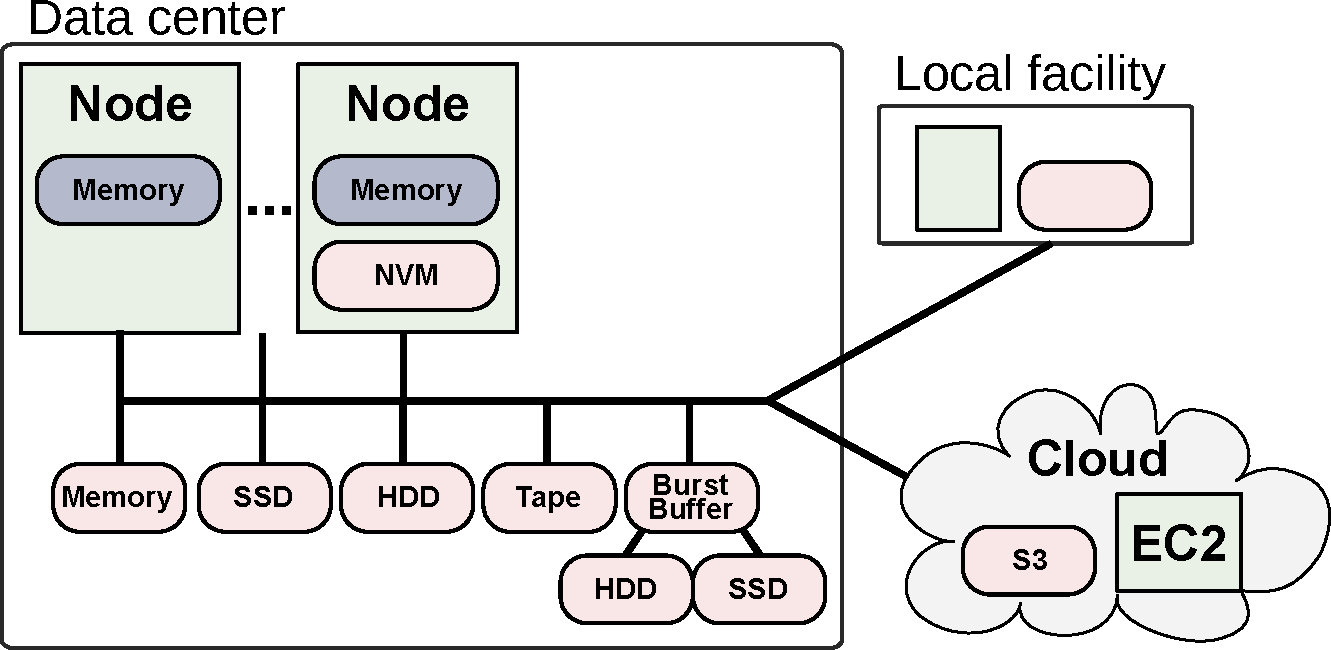
\includegraphics[width=\columnwidth]{system}
  \caption{Example Heterogeneous HPC Landscape}
  \label{fig:heterogeneous}
\end{figure}



\subsection{Experimental Planning}

Knowledge about workflow execution and overall experimental design can help to
optimize execution and environments.
From the perspective of scientists and engineers, the time-to-solution from experimental design to insight matters.
At the moment, users of public data center services supply limited information about their experiments, typically the level of detail is like "I need X CPU hours and Y storage capacity".
Still, the systems these workflows later will run cost 10 or 100 million of dollars.
Compare this to other experiments conducted in physics like the Large Hadron Collider (LHC) at CERN or the Square Kilometer Array (SKA) which may need years of planning.
While it is important to keep some freedom to explore ad-hoc experiments, we raise the question what could the HPC community achieve knowing workflows in more detail.
%Kubernetes

\subsubsection{Example Workflow}

The execution of a workflow is illustrated in \Cref{fig:workflow}.
Arrows indicate dependencies between tasks and data.
Note that we expect that the nodes are annotated with characteristics of the workflow;
data can be annotated with metadata describing its content, the expected data life cycle information, e.g., the value of data and how long should it be kept; tasks can be annotated with the information to run them and runtime.

Task\,1 needs two datasets to perform its work, it directly communicates with Task\,2 and produces Product\,1.
Most of the workflow can run automatically except the manual quality control of the products and the final data usage of Product\,3 at the end.
The last step represents the typical uncertainty of data reuse, when this workflow is created it is unclear how Product\,3 will be used further, it is apparent that it will be.
Further workflows that use the data may be created similarly and use the product as input.

\begin{figure}[b]
  \centering
  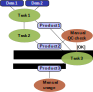
\includegraphics[width=0.75\columnwidth]{workflow}
  \caption{Example High-Level Workflow without Characteristics}
  \label{fig:workflow}
\end{figure}




\section{NGI Vision}

Our vision for Next Generation Interfaces is a new approach for data management and data-driven computation.
%\paragraph{Data Model}
NGI tackles the challenge of storage and data-flow computation in an holistic way, accepting that data storage is only aiding the goal of generating insight.
Besides providing a typical abstract data model, NGI treats domain metadata\footnote{Therewith, we mean non-technical information about the data, for instance, the name of an experiment.}, workflows, and information lifecycle management as first-class citizens.
This user information is exploited by smart components of NGI which target to exploit heterogeneous system landscapes.
To describe the features and benefits of the approach further, we sketch the user and system perspective in the following, as this highlights how we believe we should work in the 21st century.
The vision covers not only HPC but spans cloud, enterprise, and personalized IT.

\subsection{User Perspective}

\newcommand{\bnf}[1]{\textless #1\textgreater}

From the users perspective, the interface and system matches the core requirements and expectations including reliability, availability, and usability.

\paragraph{Data model:} the data model is derived from state-of-the-art solutions like HDF5.
However, it abstracts from data localization and low-level concepts like files and directories and puts its focus on data organization and data structures.
The integration into applications is shown in \Cref{fig:ngilayers}.
Applications may utilize the NGI API directly, or utilize existing middleware\footnote{Which typically won't be able to utilize the full set of features.}.
From the perspective of a developer of middleware or an application like web publishing, NGI provides a common feature set that reduces the amount of code replication inside domain-specific solutions.


\paragraph{Namespace:} data is accessed using information from the domain metadata, i.e., similar to using methods of data indexing services.
The system won't relying on a hierarchical namespace but a dynamic mapping to the POSIX namespace can be provided to enable compatibility for POSIX applications.
For example, a user may decide to see a hierarchy like an experiments \bnf{Date}/\bnf{Name}/\bnf{Timestep}/\bnf{Variable}.

\paragraph{Workflow specification:} the user defines a workflow describing the intentions of data manipulation and the data lifecycle including manual (user) involvement in the data processing.
This also includes the definition of constraints, for instance, deadlines for the generation of the final data products (insight).
Workflows can be defined using arbitrary tools including Python.
Note that a user does not provide a concrete mapping to system or infrastructure but expects that the system derives an optimized execution plan that covers heterogeneous infrastructures.
It does not matter where data is processed and if and where data is stored but only that the desired result with all constraints is met.
Workflows are recorded and data lineage of data products can be inspected by the user upon demand allowing to reproduce and validate correct execution of experiments.


\paragraph{Behavioral contracts:}
Besides the core characteristics, users expect the execution of their workflows under constraints (including cost and time constraints).
The system is expected to always show the expected characteristics and shield the user from system-specifics and undesired events (like faults or data loss).
The characteristics may improve over time, for instance, by expanding hardware capabilities, but the user won't have to change their workflow specification.
Still, for expert users, tools for introspecting system state and decision making are  provided.

\paragraph{Prescriptive analysis:} a toolset for users and administrators allows to explore scenarios.
Similarly, to an SQL Explain statement, this provides an unprecedented level of introspection, for instance, to predict the runtime or execution costs of a workflow on a given system.
Sharing the workflow description to vendors result in predictions for runtime and costs.
The ecosystem may also prescribe alternative systems to use, e.g., this part of the workflow will be run on data center A and this part on cloud provider B.



\subsection{System Perspective}

An implementation of the NGI API exploits the user-supplied information and system characteristics intelligently to meet the user expectations and smartly use heterogeneous compute and storage landscapes.
It is expected that machine learning techniques will be applied to serve the individual aspects and evolve the systems over time.

\paragraph{Awareness:}
the system knows and understands user metadata and the overarching workflows (with the user intentions).
It is self-aware, knowing the nominal characteristics of the hardware and software components, constantly comparing the system and workflow state with the expectations to perform mitigating actions to heal deviations.
At best, each individual hardware component would ship with a behavioral model that can be integrated hierarchically up to a global system model.
With behavioral models we not only mean performance models but reliability and cost-models as well.

\paragraph{Resource management:}
the system is in charge to manage and provision the available hardware resources autonomously.
Ultimately, it aims to utilize the individual characteristics of heterogeneous compute and storage landscapes by utilizing intelligent scheduling.
Data placement and localization is beyond mere tiering strategies, parts of data may be placed on certain storage technology, or replicated in different representations across storage characteristics.
Therewith, serving different access patterns and workflows at the same time.
Naturally, the system will replicate (expand) upon the availability of storage space while reducing redundancy under shortage of space.

\paragraph{Liquid computing:}
the system is in charge to manage and provision the available hardware resources autonomously and to assign compute and storage resources to tasks.
Therewith, it may use, e.g., GPU, CPU, and in-network computing capabilities to serve pieces of a single workflow.
We call this concept \textbf{liquid computing} as the compute resources are dynamically provisioned and assigned while data flows through the system it is processed.
Naturally, processing closer to the data sources is likely to improve system throughput.


\paragraph{Scheduling:}
supplied with user workflows and their characteristics, the system derives execution plans for the computation and make data placement decisions that aim to utilize the available hardware resources.
As NGI is in charge in both, it may decide to trade computation vs. storage capacity; for example, enabling automatic recomputation of intermediate states.
Similarly, the scheduler may decide to couple subsequent steps of a workflow directly without storing intermediate data products on persistent storage.
Data might be replicated but enables the system to rerun parts of the workflow in case of a data loss.

The automatic scheduling is key to efficient processing and will allow constant improvement without forcing user to adjust their workflows.
In most cases, individual resources are not used exclusively by a single task but QoS methods ensure that constraints of workflows are met.


\paragraph{Extensible ecosystem:}
the hardware and software landscape will be open allowing to connect solutions from different vendors.
Imagine that a certain class of workflows performs inefficiently on a given infrastructure indicating a crucial processing or storage capability is missing.
Adding new capabilities or resources to the system will allow the scheduler to use them in subsequent user-workflows similarly easy to an appliance.



\begin{figure}[b]
  \centering
  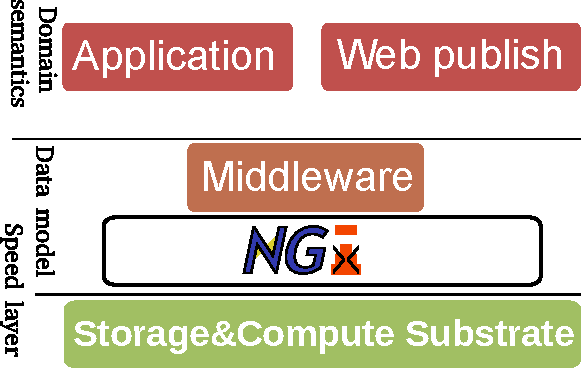
\includegraphics[width=0.75\columnwidth]{layers-ngi}
  \caption{Layers with NGI}
  \label{fig:ngilayers}
\end{figure}




\section{Community Strategy}

We are in the process to establish the NGI Forum that curates the development of the APIs.
The process will share the idea with the successful MPI Forum, the approach is sketched in \Cref{fig:standardization}.
Members are experts from domain science, industry and data centers and form the bodies
which activity is lead by the elected steering board.
Topic-specific workgroups and committees develop the standard (data model and APIs) driven by relevant use-cases encompassing the span from workflows to code snippets.
Ultimately, we will support the creation of a reference implementation based on state-of-the-art technology that demonstrates the approach on the use-cases.
We are aware that this endeavor is challenging; therefore, we won't expect that NGI 1.0 will include every feature.
%We will settle on the set of features that the consortium identifies
%Similar to the way MPI 1.0 has grown, .

We expect that vendors and researchers will embrace the open ecosystem similarly to MPI and explore and contribute to the forum and its development.

\begin{figure}[b]
  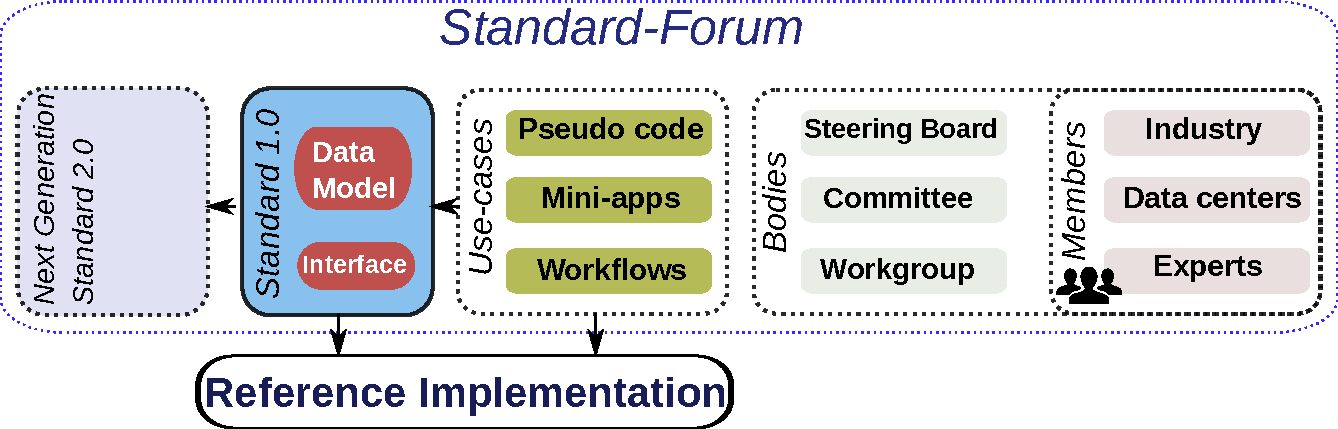
\includegraphics[width=\columnwidth]{standardization}
  \caption{Organization of the NGI Forum}
  \label{fig:standardization}
\end{figure}

\section{Conclusions}

Open ...


\includegraphics[width=2cm]{ngi-logo}

\noindent\url{https://ngi.vi4io.org}


\end{document}
